\chapter{SYSTEM ARCHITECTURE AND IMPLEMENTATION}

This chapter describes how the implementation is organised: the end-to-end
processing flow, repository layout, technology choices, and the main components
that realise static analysis and execution (type checker, interpreter, and user
interfaces). Detailed treatment of lexical analysis, the symbol table, and
parsing appears in Chapters~3 and~4; Chapter~5 presents the type-inference rules
that the type checker implements.

\section{Compiler pipeline}
The system follows a four-stage pipeline. Lexical and syntactic processing are
kept separate from semantic analysis and execution, which simplifies testing and
localises errors to the appropriate stage.

The overall flow of data through the system is shown in
Figure~\ref{fig:system-overview-pipeline}.

\begin{figure}[H]
\centering
\resizebox{\textwidth}{!}{%
\begin{tikzpicture}[
  box/.style  = {rectangle, rounded corners=4pt,
                 draw=nodeblue, fill=boxblue,
                 minimum width=2cm, minimum height=0.95cm,
                 align=center, font=\large\bfseries},
  data/.style = {rectangle, rounded corners=3pt,
                 draw=arrowgray, fill=boxgray,
                 minimum width=1.7cm, minimum height=0.85cm,
                 align=center, font=\large\itshape},
  sbox/.style = {rectangle, rounded corners=4pt,
                 draw=nodeorange, fill=boxorange,
                 minimum width=2.2cm, minimum height=0.9cm,
                 align=center, font=\large},
  pbox/.style = {rectangle, rounded corners=4pt,
                 draw=nodegreen, fill=boxgreen,
                 minimum width=26cm, minimum height=0.9cm,
                 align=center, font=\large},
  arr/.style  = {-{Stealth[length=7pt,width=6pt]},
                 line width=1.2pt, color=arrowgray},
  sarr/.style = {-{Stealth[length=7pt,width=6pt]},
                 line width=1pt, color=nodeorange, dashed},
  node distance = 0.7cm and 1cm,
]

\node[data]                (src) {Source\\Code};
\node[box,  right=of src]  (lex) {Lexer};
\node[data, right=of lex]  (tok) {Tokens};
\node[box,  right=of tok]  (par) {Parser};
\node[data, right=of par]  (ast) {AST};
\node[box,  right=of ast]  (tck) {Type\\Checker};
\node[data, right=of tck]  (chk) {Checked\\AST};
\node[box,  right=of chk]  (itp) {Interpreter};
\node[data, right=of itp]  (out) {Output};

\node[sbox, below=1.5cm of tck] (sym) {Symbol\\Table};

\node[pbox, below=0.8cm of sym] (pip)
  {\texttt{pipeline.py}\quad---\quad shared by CLI, desktop UI, and test suite};

\draw[arr] (src) -- (lex);
\draw[arr] (lex) -- (tok);
\draw[arr] (tok) -- (par);
\draw[arr] (par) -- (ast);
\draw[arr] (ast) -- (tck);
\draw[arr] (tck) -- (chk);
\draw[arr] (chk) -- (itp);
\draw[arr] (itp) -- (out);

\draw[sarr] (tck.south) -- (sym.north)
  node[midway, right=3pt, font=\normalsize\itshape, color=nodeorange] {builds};
\draw[sarr] (sym.east) -| (chk.south);

\end{tikzpicture}%
}
\caption{Front-end and interpreter pipeline overview.}
\label{fig:system-overview-pipeline}
\end{figure}

Source characters are scanned by the lexer into a token stream. The parser
consumes tokens and builds an AST that reflects program structure (expressions,
statements, and control flow). The type checker then walks the AST, populates and
uses the symbol table, infers types, and validates scope and type rules. Only
programs that pass the type checker proceed to interpretation. The interpreter
evaluates the checked tree using ordinary Python values; it does not re-run the
type rules, since correctness at runtime is guaranteed by the prior static pass.
All four stages are orchestrated through \texttt{pipeline.py}, which is shared
by the command-line runner, the desktop UI, and the test suite.

\subsection{End-to-end pipeline walkthrough}

The following example traces the complete execution of a three-statement program
through all four pipeline stages, illustrating the correspondence between source
text, tokens, abstract syntax tree, inferred types, and runtime output.

\textbf{Source program:}
\begin{lstlisting}
a = 3;
b = 4;
print(a + b);
\end{lstlisting}

\textbf{Stage 1 --- Lexer output (token stream):}
\begin{lstlisting}
IDENTIFIER     'a'     line 1, col 1
ASSIGN         '='     line 1, col 3
INT_LITERAL    '3'     line 1, col 5
SEMICOLON      ';'     line 1, col 6
IDENTIFIER     'b'     line 2, col 1
ASSIGN         '='     line 2, col 3
INT_LITERAL    '4'     line 2, col 5
SEMICOLON      ';'     line 2, col 6
PRINT          'print' line 3, col 1
LPAREN         '('     line 3, col 6
IDENTIFIER     'a'     line 3, col 7
PLUS           '+'     line 3, col 9
IDENTIFIER     'b'     line 3, col 11
RPAREN         ')'     line 3, col 12
SEMICOLON      ';'     line 3, col 13
EOF                    line 3, col 14
\end{lstlisting}

\textbf{Stage 2 --- Parser output (abstract syntax tree):}
\begin{lstlisting}
Program  [3 statement(s)]
    Assign  'a'  =
        Literal  3  (int)
    Assign  'b'  =
        Literal  4  (int)
    Print
        BinaryOp  '+'
            left:
                Identifier  'a'
            right:
                Identifier  'b'
\end{lstlisting}

\textbf{Stage 3 --- Type checker output (inferred type environment):}

\begin{table}[H]
\centering
\small
\begin{tabular}{@{} ll @{}}
\toprule
\textbf{Name} & \textbf{Inferred type} \\
\midrule
\texttt{a}     & \texttt{Integer} \\
\texttt{b}     & \texttt{Integer} \\
\bottomrule
\end{tabular}
\end{table}

\noindent The symbol table records only named symbols (\texttt{a} and \texttt{b}).
The type checker additionally infers that the sub-expression \texttt{a + b}
has type \texttt{Integer} (Integer $+$ Integer $\rightarrow$ Integer) during
AST traversal, but sub-expression types are not stored in the symbol table.

\textbf{Stage 4 --- Interpreter output:}
\begin{lstlisting}
7 : Integer
\end{lstlisting}

The example demonstrates the full data flow: source characters are tokenised by
the lexer, structured into an AST by the parser, validated and annotated by the
type checker, and finally evaluated by the interpreter to produce typed output.

\subsection{Entry points and shared pipeline}
All stages are orchestrated by \texttt{components/pipeline.py}, which is shared
by the command-line runner, the desktop UI, and the test suite.
From the project root, the CLI and desktop UI can be launched as follows:

\begin{lstlisting}
# macOS / Linux
python3 main.py       # run CLI (built-in sample or script file)
python3 ui.py         # open desktop workbench

# Windows
.\venv\Scripts\python.exe main.py
.\venv\Scripts\python.exe ui.py
\end{lstlisting}

\noindent The CLI prints the four pipeline stages in order: tokens, AST text,
type table, and execution output. The desktop workbench uses the same pipeline
internally, presenting each stage in a separate tab for inspection.

\section{Project structure}
The main source files and their responsibilities are summarised in
Table~\ref{tab:main-source-files}.

\begin{table}[H]
\centering
\caption{Main source files}
\label{tab:main-source-files}
\begin{tabular}{ll}
\toprule
File & Responsibility \\
\midrule
\texttt{main.py} & Command-line runner for sample code or a script file \\
\texttt{ui.py} & Desktop UI for editing and running a script \\
\texttt{components/tokens.py} & Token classes and token categories \\
\texttt{components/lexica.py} & Lexical analysis \\
\texttt{components/ast\_nodes.py} & AST node definitions \\
\texttt{components/parser.py} & Recursive-descent parser \\
\texttt{components/ast\_printer.py} & AST renderer for debugging and reporting \\
\texttt{components/symbol\_table.py} & Scoped symbol table and semantic types \\
\texttt{components/type\_checker.py} & Static type checker and inference \\
\texttt{components/interpreter.py} & Tree-walking interpreter \\
\texttt{components/pipeline.py} & Shared pipeline for CLI, UI, and tests \\
\bottomrule
\end{tabular}
\end{table}

\section{Technology stack}
The project uses Python and standard-library tools only
(Table~\ref{tab:technology-stack}).

\begin{table}[H]
\centering
\caption{Technology stack}
\label{tab:technology-stack}
\begin{tabular}{ll}
\toprule
Tool & Purpose \\
\midrule
Python 3.10+ & Core implementation language \\
\texttt{dataclasses} & AST and runtime helper structures \\
\texttt{tkinter} & Desktop graphical interface \\
\texttt{unittest} & Automated testing \\
\bottomrule
\end{tabular}
\end{table}

\section{Type checker}
The \texttt{TypeChecker} class implements the inference and checking rules
described in Chapter~5. It traverses the AST before execution, uses the symbol
table to record variable and function information, infers types on first
assignment, validates arithmetic and comparison expressions, enforces Boolean
conditions for control flow, infers function parameter types from the first call
(or from body usage for uncalled functions), and infers function return types
from \texttt{return} statements. Programs that
fail these rules are rejected before interpretation.

\subsection{Scope of the implemented type system}
In scope terms, this component turns a syntactically valid AST into a
semantically valid program:

\begin{itemize}
	\item static typing rules for arithmetic, comparison, assignment, control
	flow, and functions,
	\item type checking for expressions and statements,
	\item variable type inference from first assignment,
	\item function parameter inference from the first call (or from body usage for uncalled functions),
	\item function return type inference from \texttt{return} statements,
	\item source-positioned type errors when a program violates a typing rule.
\end{itemize}

\section{Interpreter}
The interpreter is a tree-walking evaluator over the checked AST. It maintains
nested runtime environments for variables and function calls. Assignments write
through the current or nearest enclosing scope; \texttt{if} selects a branch;
\texttt{while} repeats until its condition becomes false; function calls bind
arguments by value and return through an internal return mechanism.

The built-in \texttt{print()} function outputs both value and runtime type.
All four types are supported:

\begin{lstlisting}
print(42);       (* 42 : Integer       *)
print(3.14);     (* 3.14 : Float       *)
print(true);     (* true : Boolean     *)
print("plc");   (* "plc" : String     *)
\end{lstlisting}

\subsection{Scope of the implemented runtime}
The runtime stage provides observable behaviour and integrates with the shared
pipeline:

\begin{itemize}
	\item assignment execution,
	\item \texttt{if} execution,
	\item \texttt{while} execution,
	\item function execution with value parameter passing,
	\item \texttt{print()} execution with immediate output,
	\item execution behind the same \texttt{run\_pipeline} path used by the CLI,
	UI, and tests.
\end{itemize}

\section{Graphical user interface}
The desktop workbench (\texttt{ui.py}) is implemented with Python's
\texttt{tkinter} standard library and requires no additional dependencies.
The window is titled \textit{125970-126690-126687-Ass2-PLC} and
opens at $1200 \times 760$ pixels in a horizontal split layout.

\textbf{Toolbar.}  A top toolbar provides three buttons --- \textit{Open
Script}, \textit{Run}, and \textit{Clear Output} --- and a right-aligned
status label that reports \textit{Ready}, a loaded filename, or \textit{Run
failed}.

\textbf{Left panel (source editor).}  A monospaced \texttt{Text} widget
with both horizontal and vertical scrollbars allows the user to enter or
paste arbitrary source code. The \textit{Open Script} button populates the
editor from a file. The editor is pre-loaded with the built-in sample program
on first launch.

\textbf{Right panel (output tabs).}  A \texttt{Notebook} widget presents
five tabs, each backed by a scrollable read-only \texttt{Text} widget with
both horizontal and vertical scrollbars:
\begin{itemize}
  \item \textit{Execution Output} --- the \texttt{print()} values produced
        by stage~4, formatted as \texttt{value : Type}. The type label is
        determined at runtime by inspecting the Python type of the evaluated
        value; because the type checker guarantees correctness before execution,
        this always agrees with the statically inferred type;
  \item \textit{Tokens} --- the token stream from stage~1, one token per line
        with type, lexeme, and source position;
  \item \textit{AST} --- the indented tree text from stage~2;
  \item \textit{Type Table} --- the symbol table from stage~3 showing each
        name, kind, inferred type, initialisation state, and parameter list;
  \item \textit{Errors} --- populated only when a pipeline stage fails;
        shows the error message (e.g.\ \texttt{[line~2, col~5] TypeError: \ldots}).
        On a successful run this tab is cleared automatically.
\end{itemize}

\textbf{Error handling.}  If any pipeline stage raises an exception, the
error message is written exclusively to the \textit{Errors} tab and the
remaining tabs are cleared. No modal dialogs are used, so the user can edit
and rerun without dismissing a popup.

\textbf{Keyboard shortcuts.}  \texttt{F5} and \texttt{Ctrl+Enter} are both
bound to the \textit{Run} action, allowing rapid edit-run cycles without
reaching for the mouse.

\subsection{Screenshots}
Figures~\ref{fig:ui-shots} and~\ref{fig:cli-shots} show the desktop workbench
and CLI output.

% --- UI screenshots: 2-column grid ---
\begin{figure}[H]
\centering
\begin{subfigure}[t]{0.48\textwidth}
  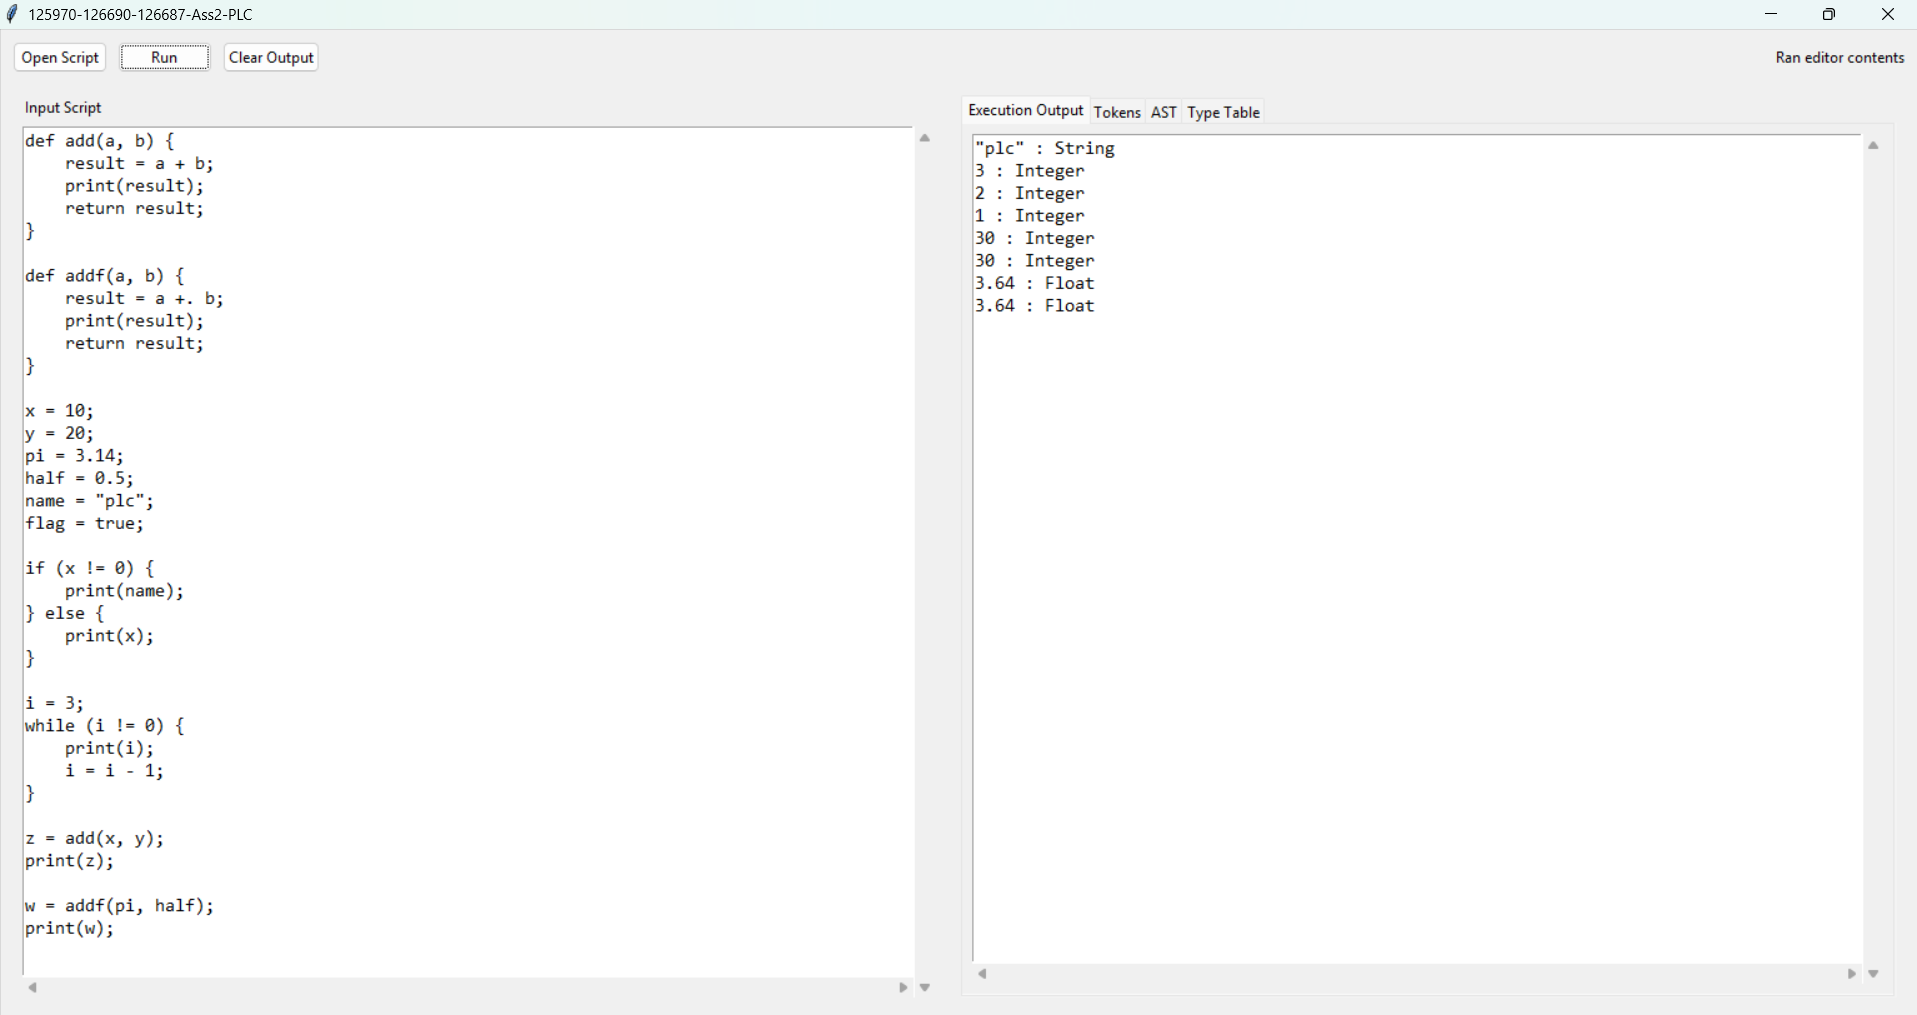
\includegraphics[width=\linewidth]{figures/ui-main.png}
  \caption{Execution Output tab.}
  \label{fig:ui-main}
\end{subfigure}\hfill
\begin{subfigure}[t]{0.48\textwidth}
  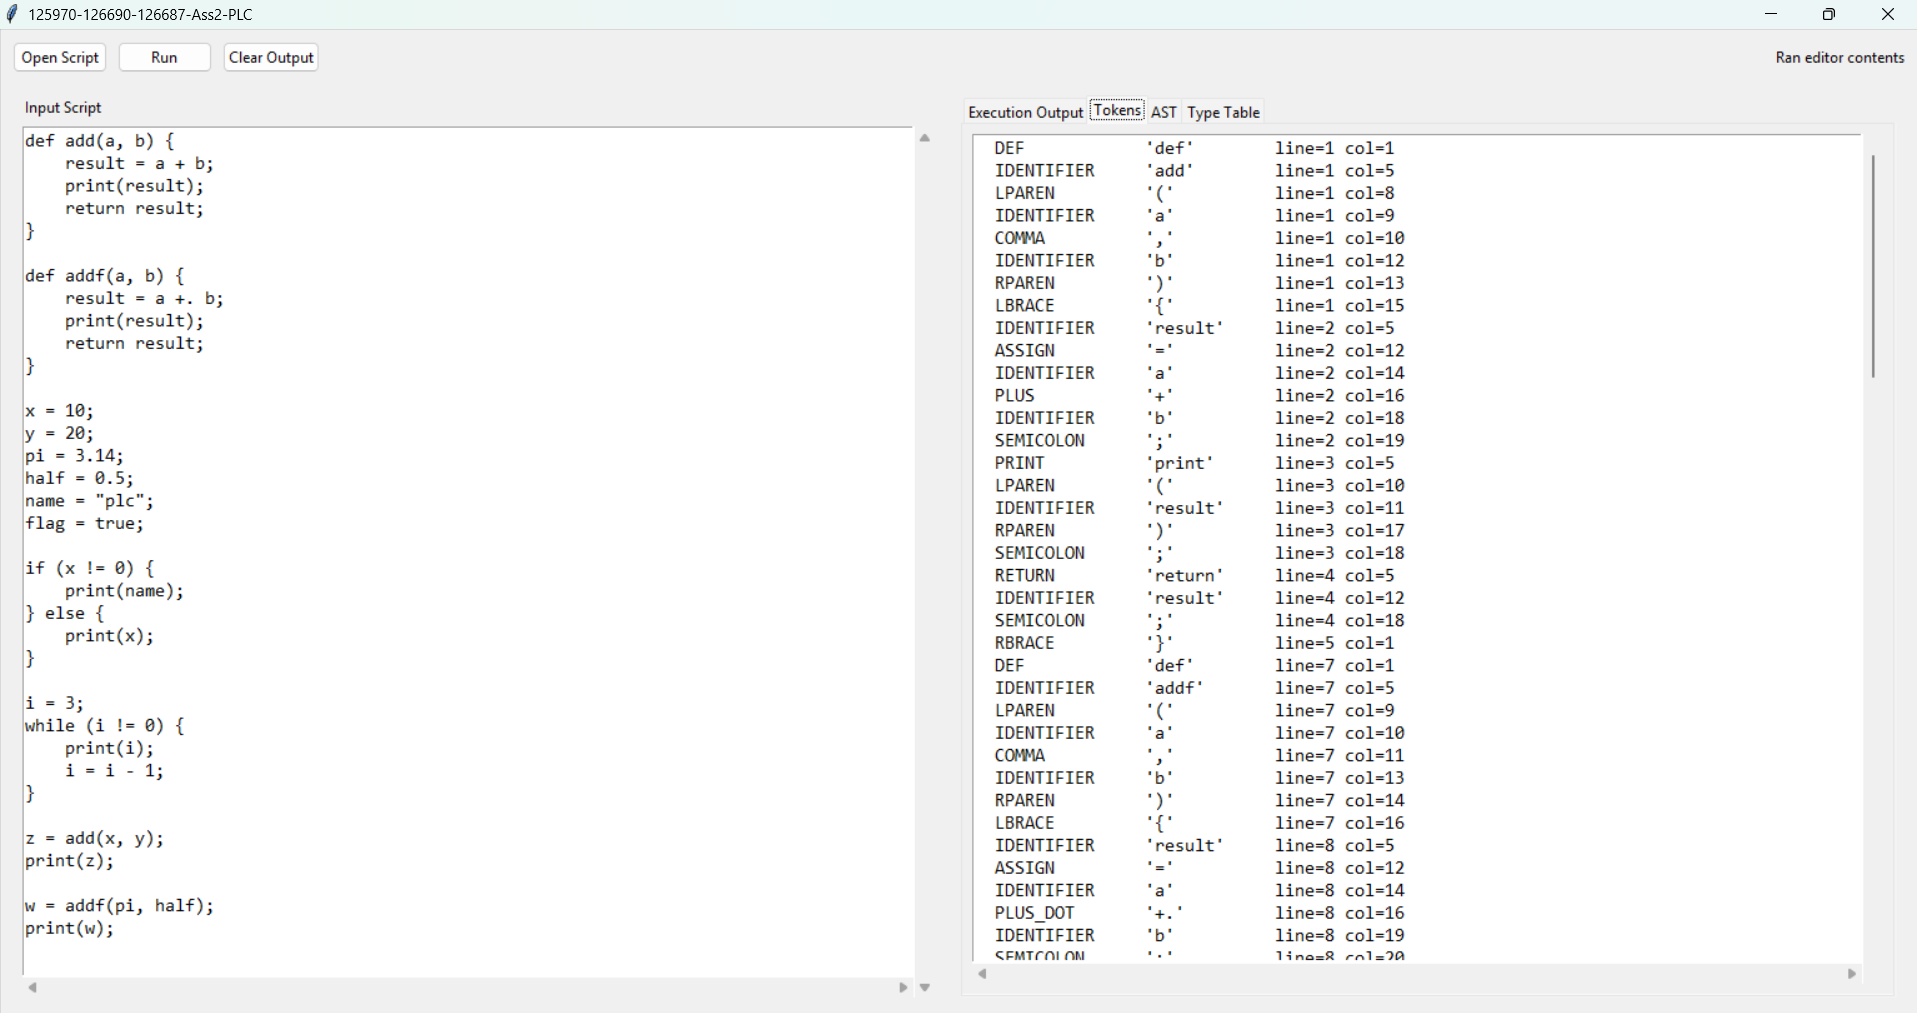
\includegraphics[width=\linewidth]{figures/ui-tokens.png}
  \caption{Tokens tab (Stage~1).}
  \label{fig:ui-tokens}
\end{subfigure}

\medskip

\begin{subfigure}[t]{0.48\textwidth}
  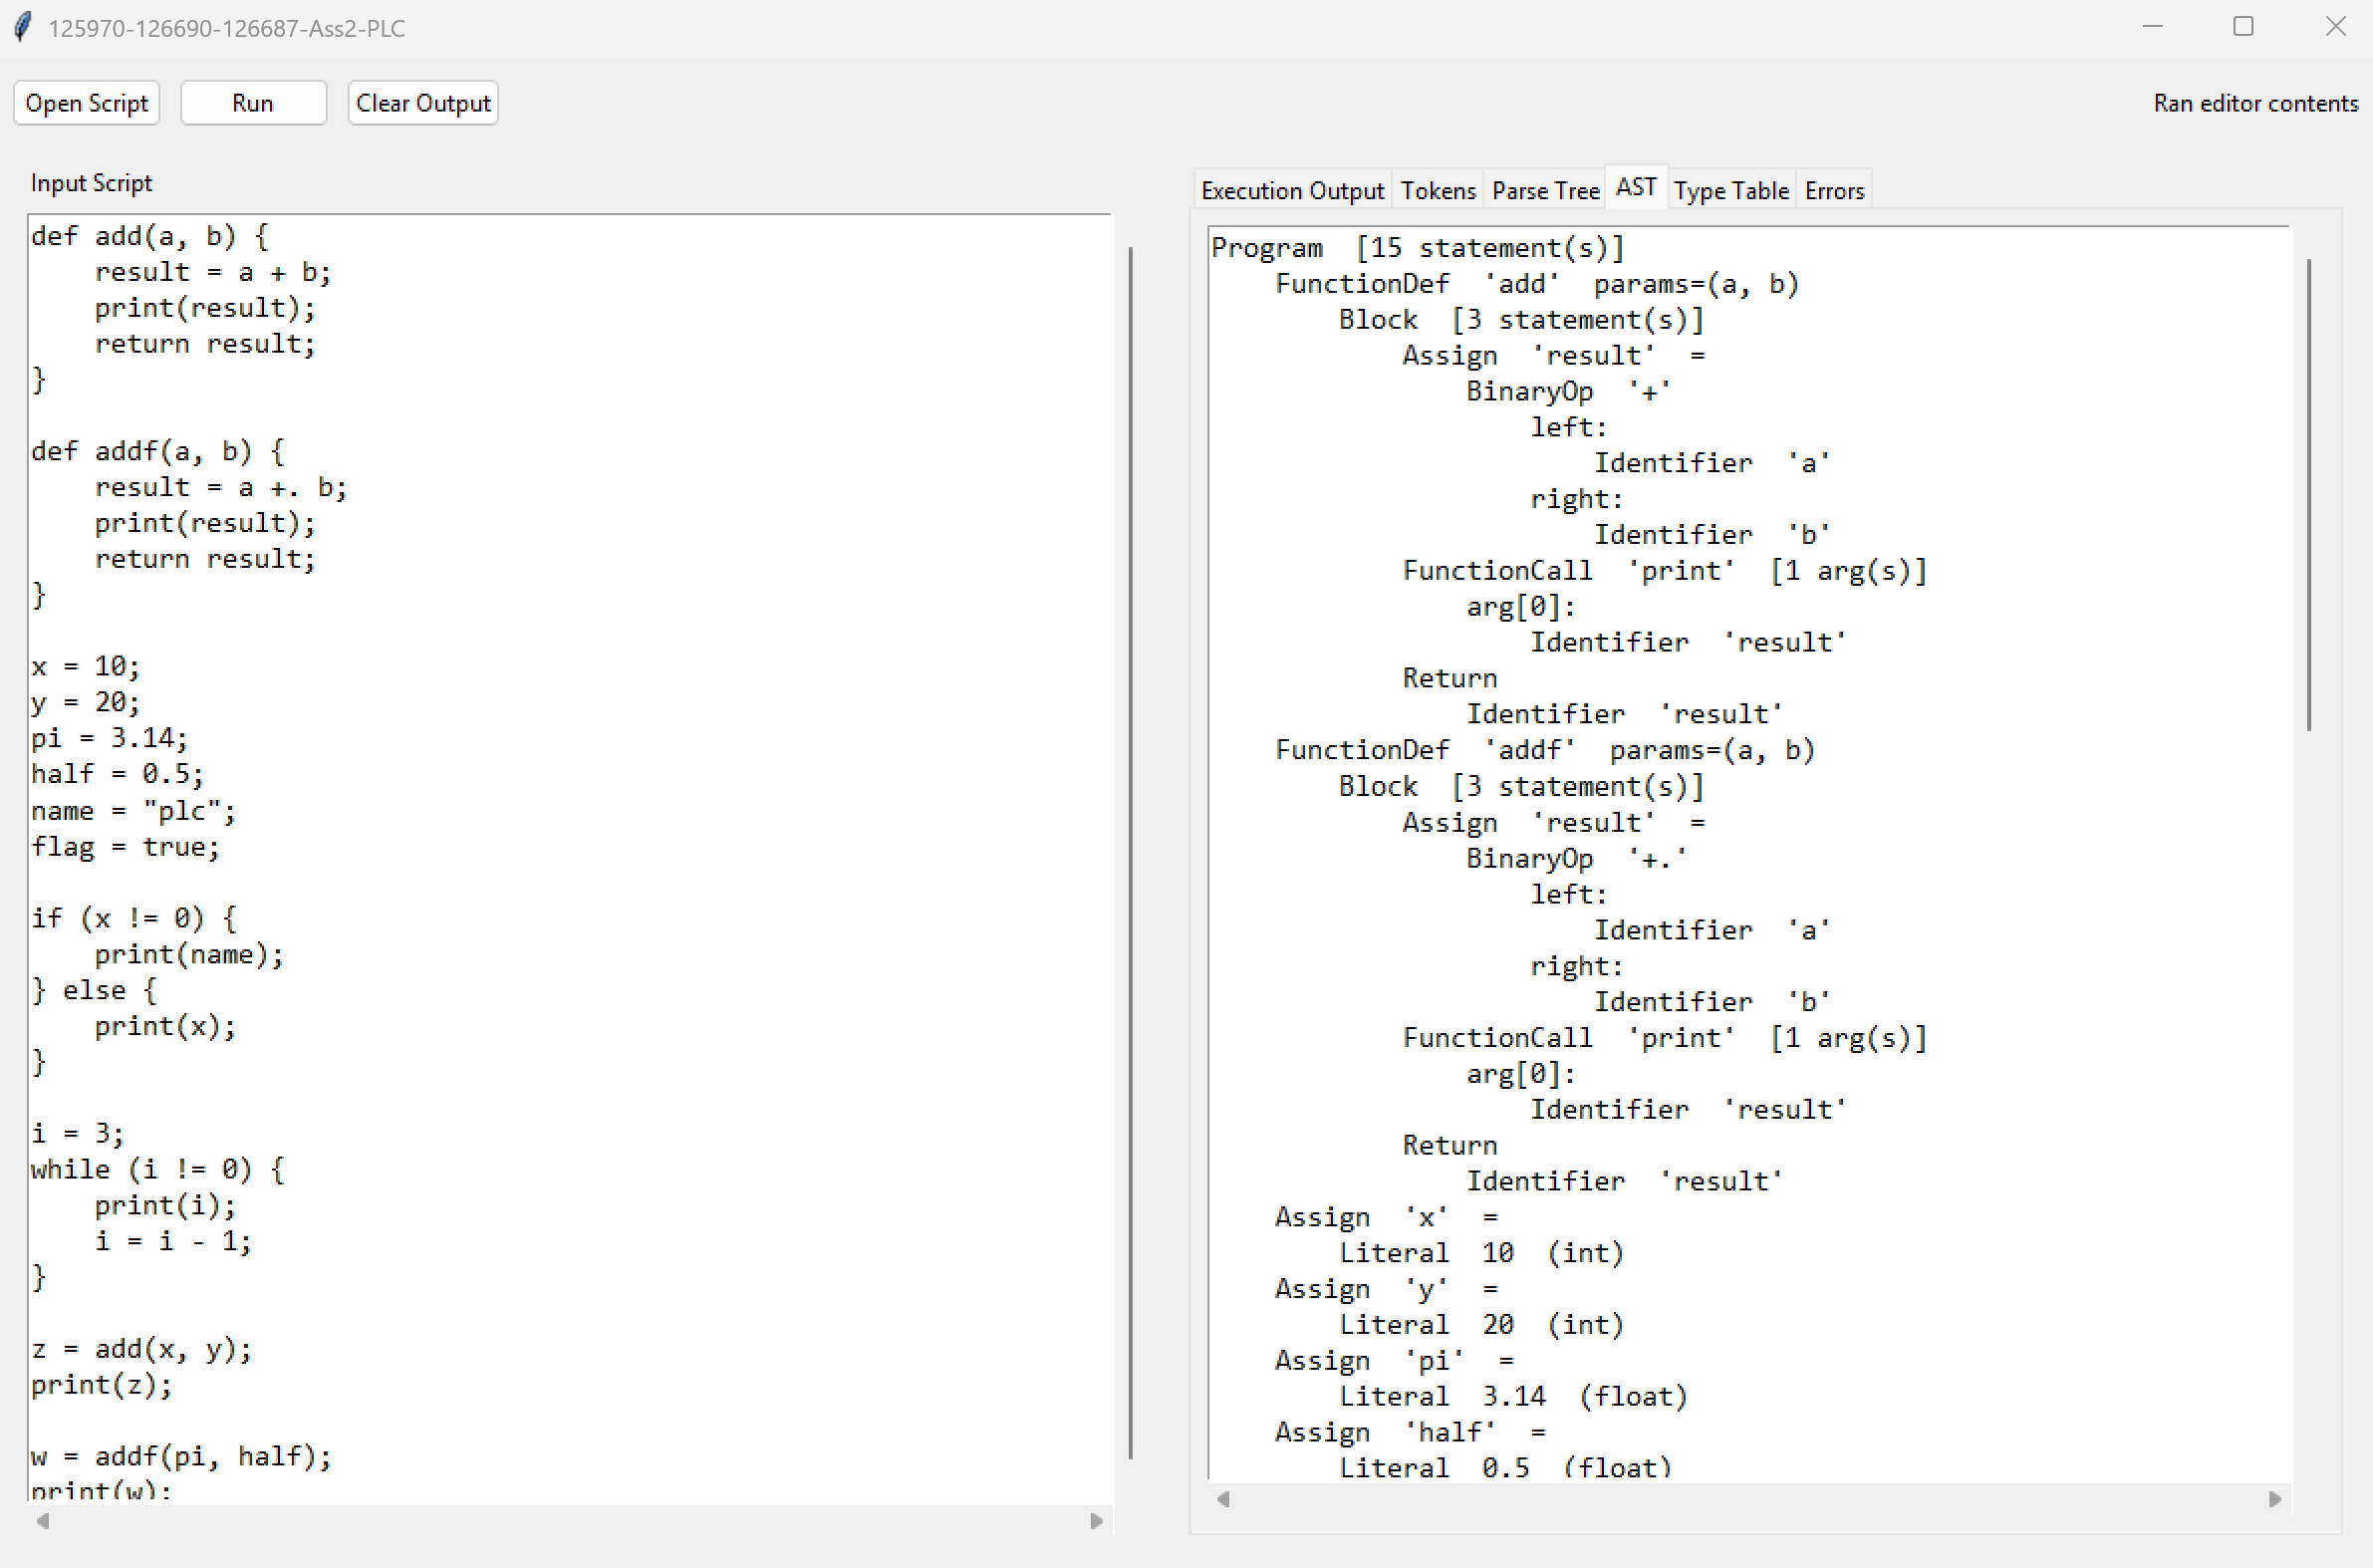
\includegraphics[width=\linewidth]{figures/ui-ast.png}
  \caption{AST tab (Stage~2).}
  \label{fig:ui-ast}
\end{subfigure}\hfill
\begin{subfigure}[t]{0.48\textwidth}
  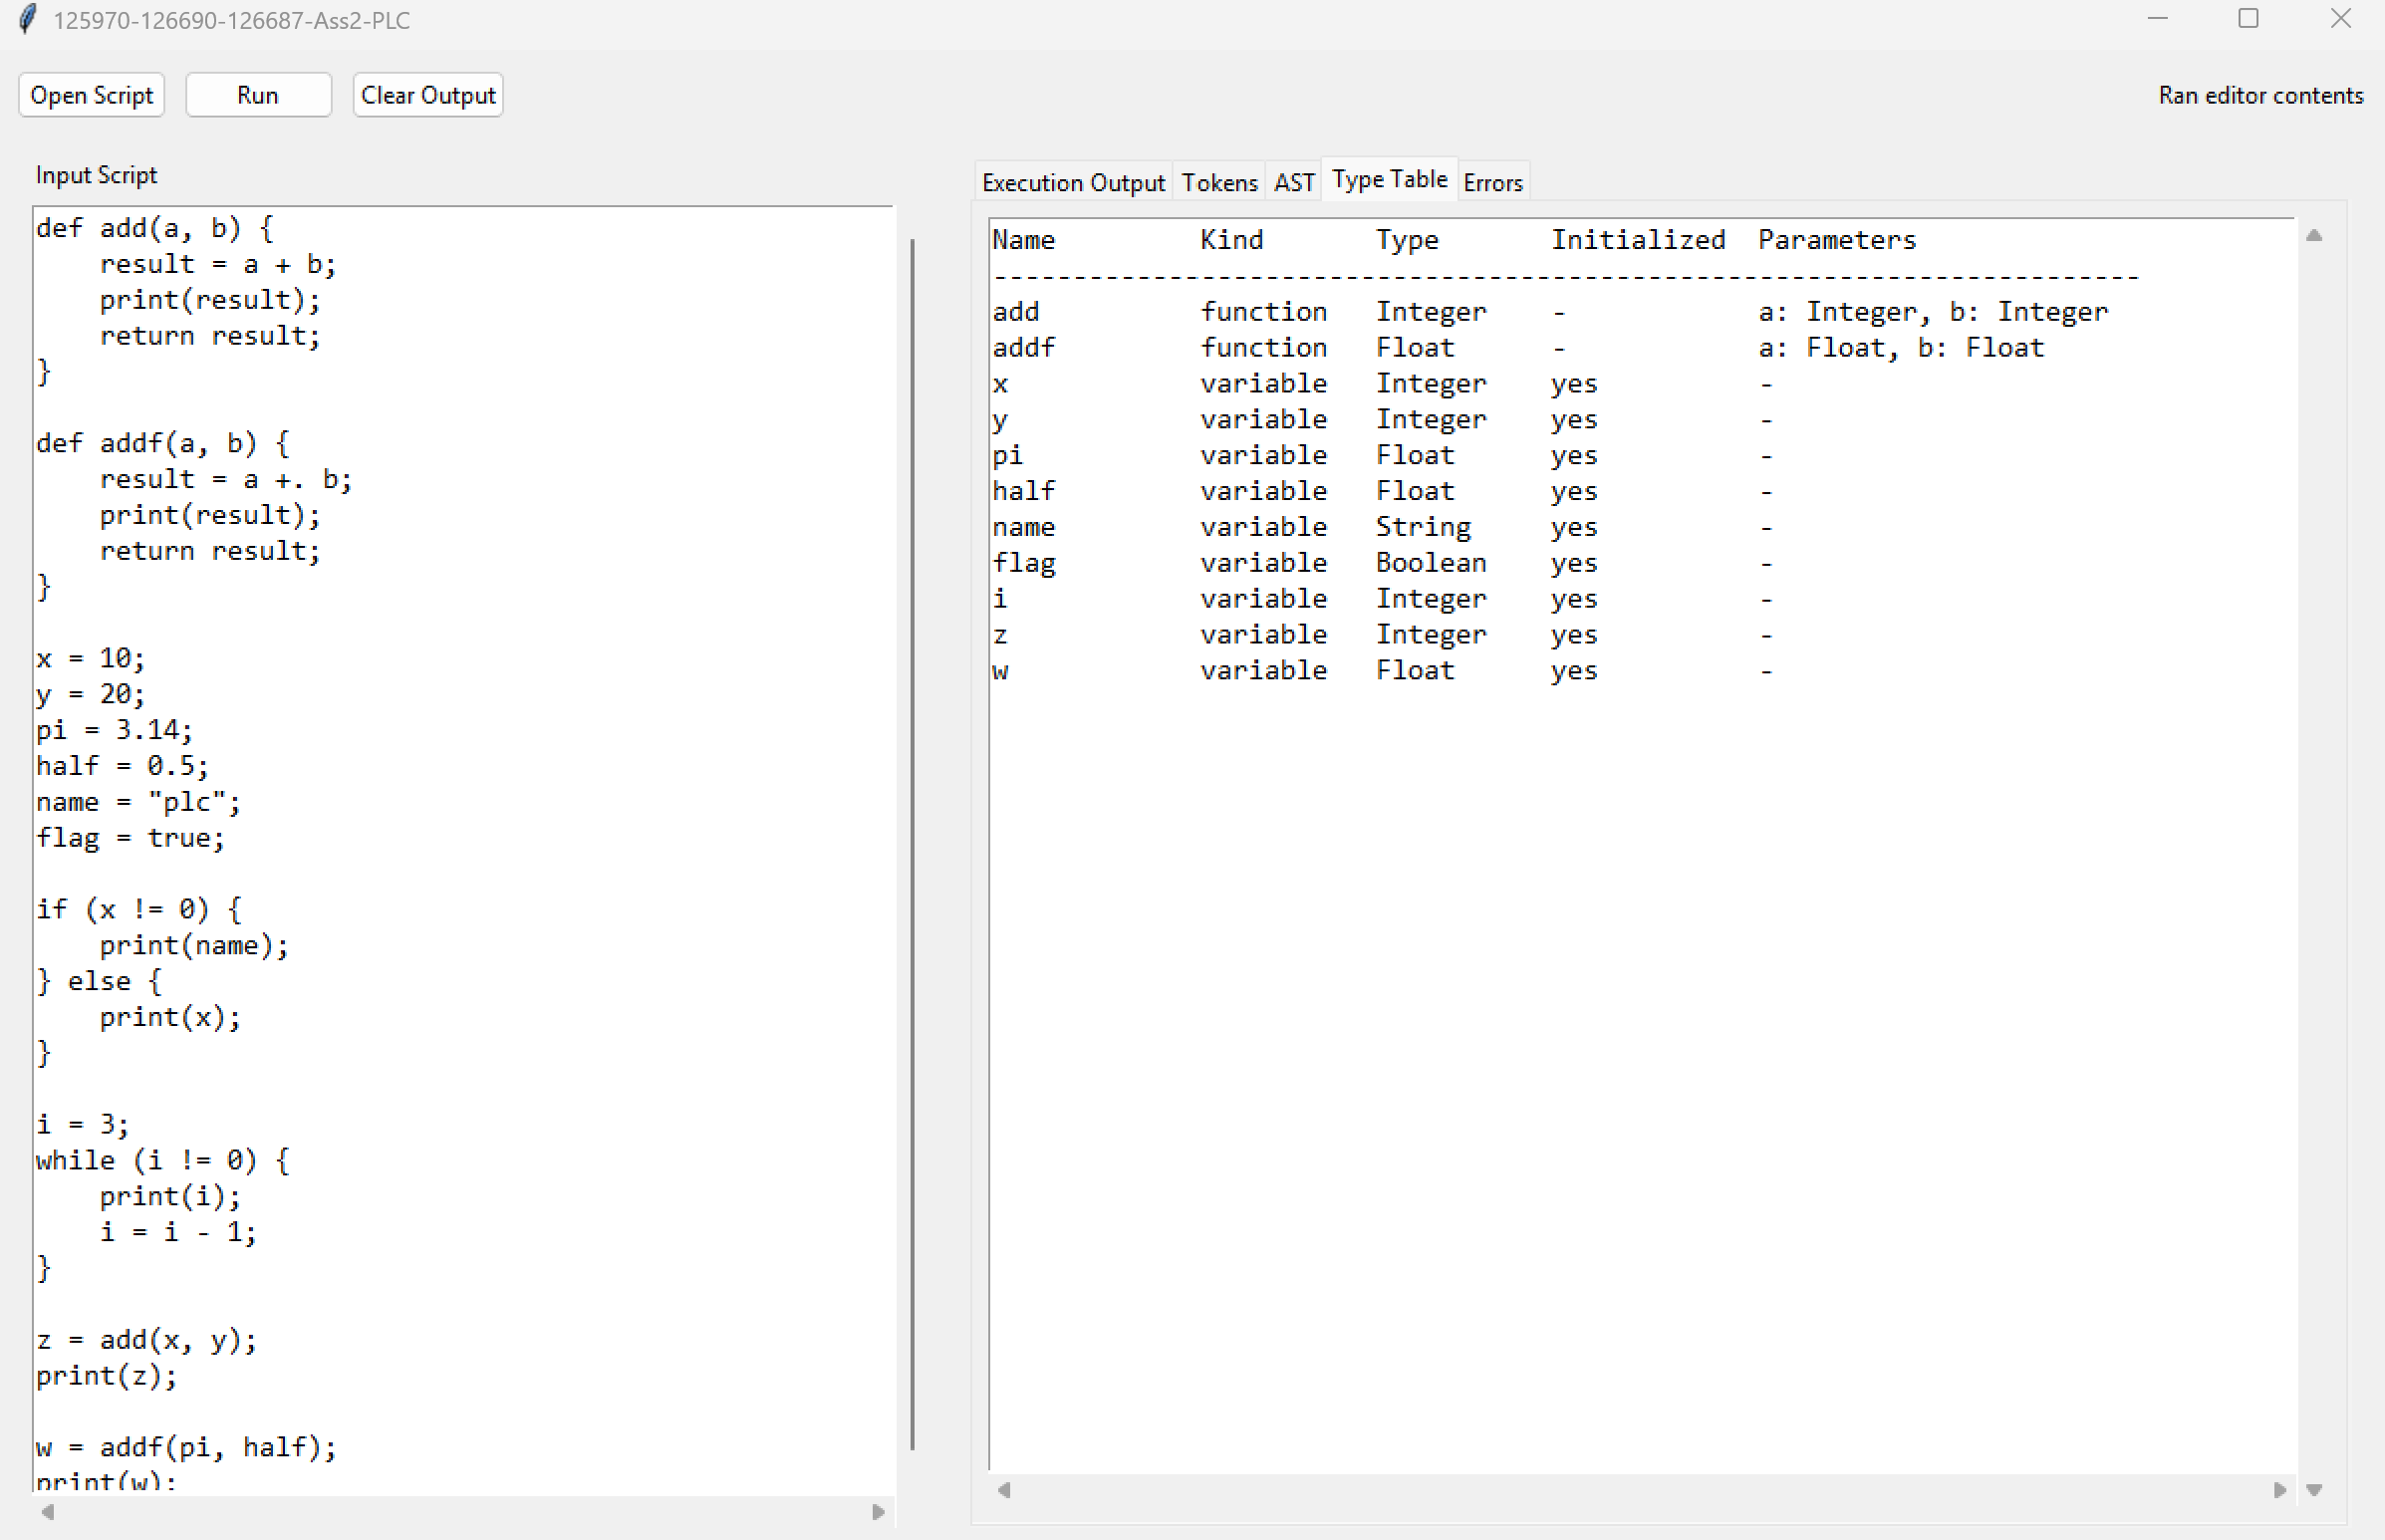
\includegraphics[width=\linewidth]{figures/ui-types.png}
  \caption{Type Table tab (Stage~3).}
  \label{fig:ui-types}
\end{subfigure}

\medskip

\begin{subfigure}[t]{0.48\textwidth}
  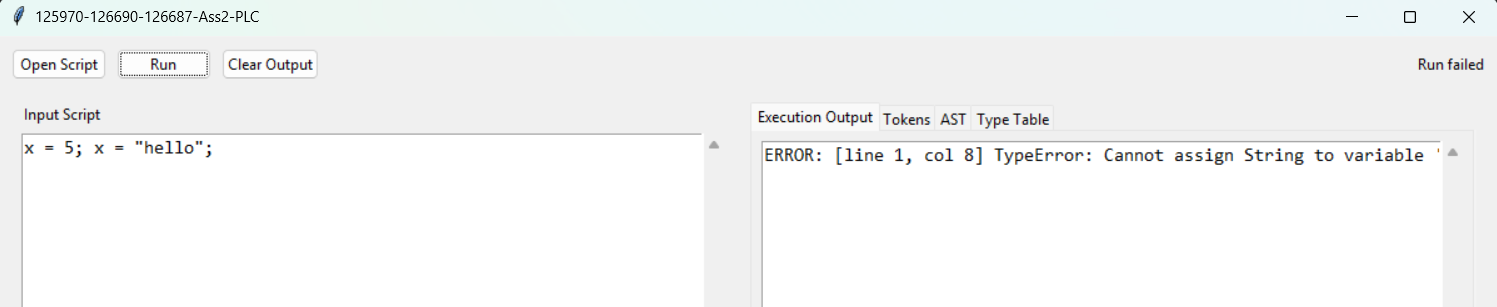
\includegraphics[width=\linewidth]{figures/ui-error.png}
  \caption{Errors tab: type error isolated from execution output.}
  \label{fig:ui-error}
\end{subfigure}
\caption{Desktop workbench --- five output tabs. Errors are reported in the
dedicated \textit{Errors} tab; all other tabs are cleared on failure.}
\label{fig:ui-shots}
\end{figure}

\section{Command-line interface}
The CLI runner (\texttt{main.py}) accepts an optional script path; without one
it runs the built-in sample and prints four labelled stages to \texttt{stdout}.
Errors are reported cleanly to \texttt{stderr}: if the specified file does not
exist, the runner prints \texttt{ERROR: File not found: <path>} and exits with
code~1. If any pipeline stage raises a language error (\texttt{LexerError},
\texttt{ParseError}, \texttt{TypeCheckError}, or \texttt{InterpreterError}),
the message is printed as \texttt{ERROR: [line~X, col~Y] <ErrorType>: <detail>}
and the process exits with code~1. In both cases no Python traceback is shown
to the user.

% --- CLI screenshots: kept on one page ---
\begin{figure}[H]
\centering
\begin{subfigure}[t]{0.48\textwidth}
  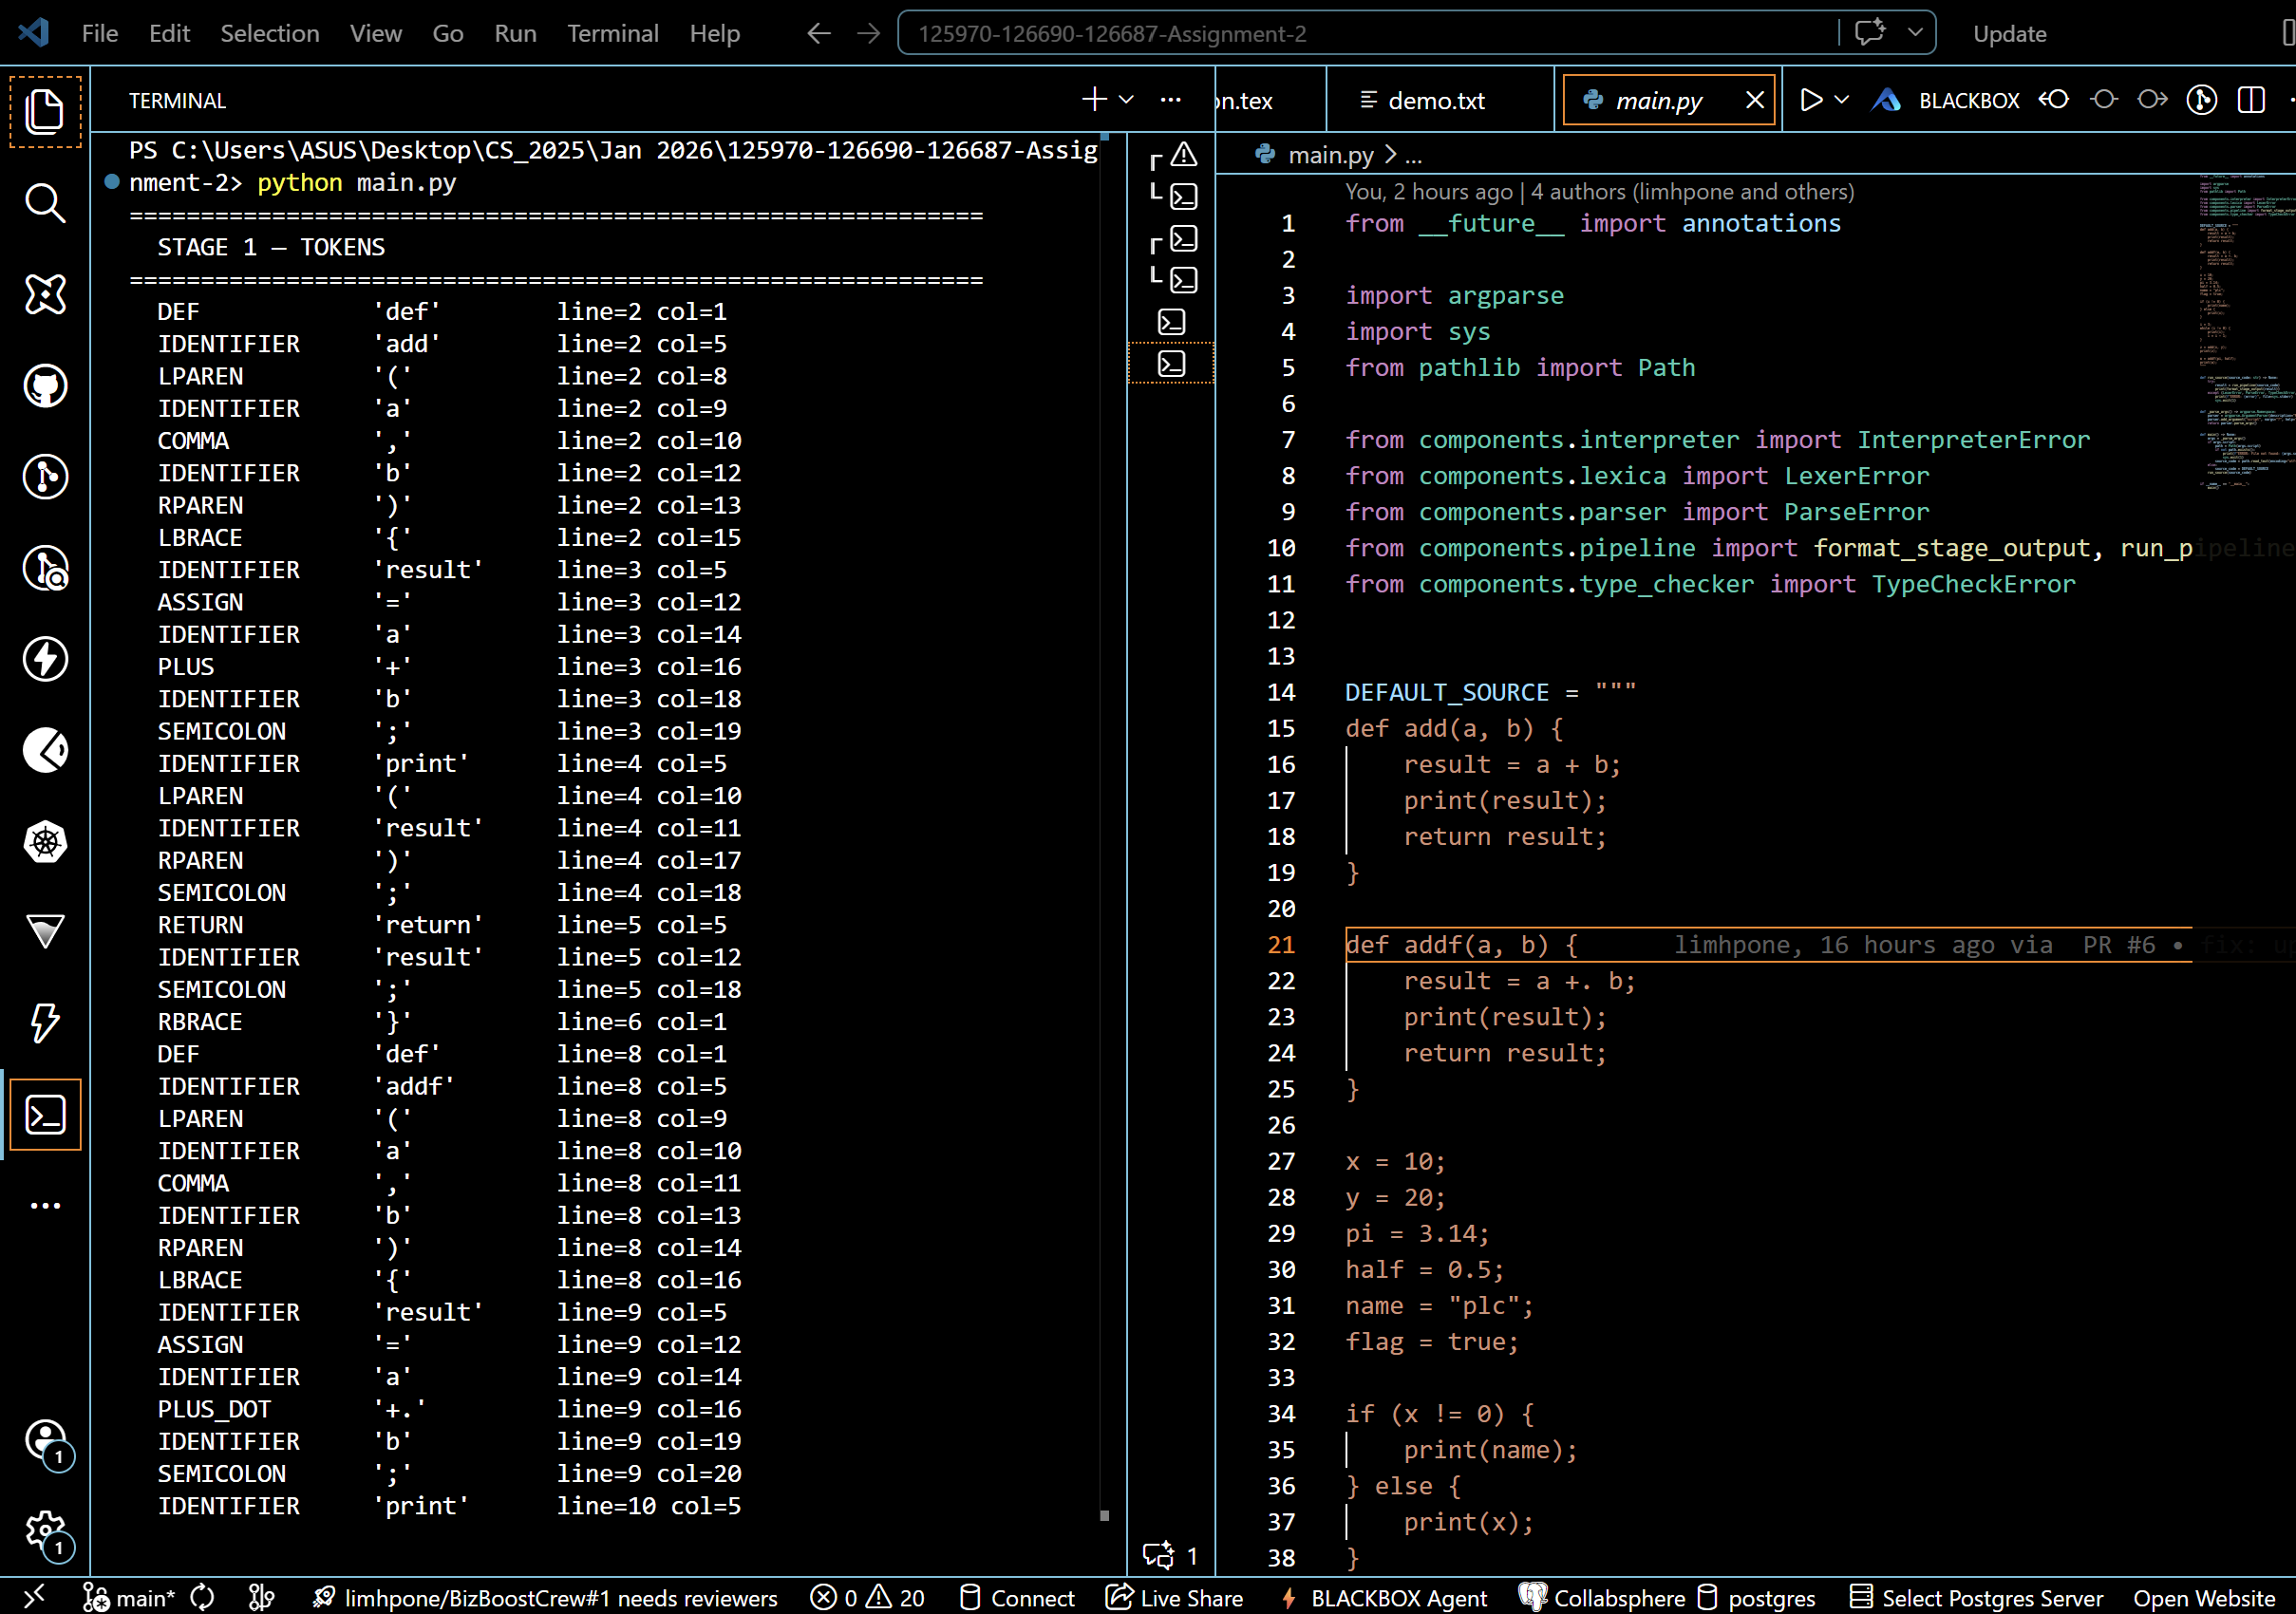
\includegraphics[width=\linewidth,height=0.32\textheight,keepaspectratio]{figures/cli-1.png}
  \caption{Stage~1: token stream.}
  \label{fig:cli-tokens}
\end{subfigure}\hfill
\begin{subfigure}[t]{0.48\textwidth}
  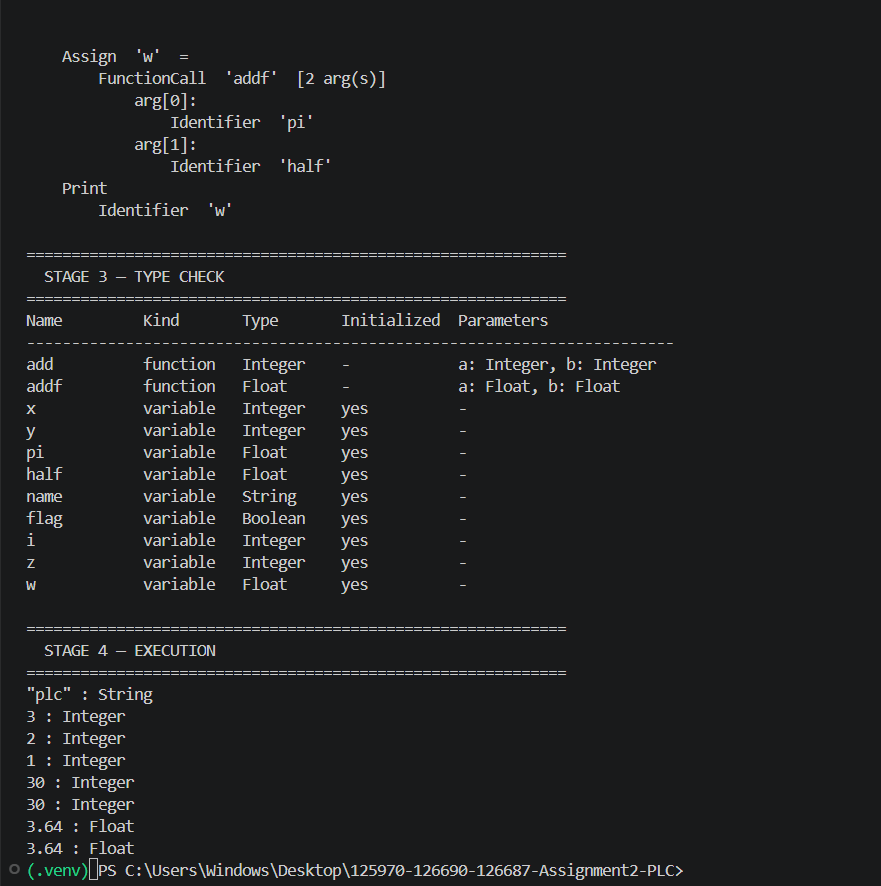
\includegraphics[width=\linewidth,height=0.32\textheight,keepaspectratio]{figures/cli-5.png}
  \caption{Stage~3 type table and Stage~4 output.}
  \label{fig:cli-exec}
\end{subfigure}
\caption{CLI run of \texttt{python main.py} on the built-in sample.}
\label{fig:cli-shots}
\end{figure}
